\chapter{Recomendaci\'on de configuraciones gr\'aficas basada en ML sobre grafos}\label{chapter:ml-on-graphs}

Los grafos son estructuras utilizadas extensivamente en la Ciencia de la Computaci\'on y otras
ramas de la ciencia debido a su capacidad de modelar estructuras basadas
en objetos y las relaciones que se establecen entre estos. Fen\'omenos
tan distintos como redes sociales, estructuras moleculares, redes de prote\'inas y
preferencias de usuarios pueden ser modelados mediante grafos.

En la actualidad los grafos desempe\~nan un rol fundamental en el
aprendizaje de m\'aquinas. Se han dise\~nado muchos sistemas para hacer predicciones o descubrir patrones dentro
de datos representados con grafos. Por ejemplo, recomendar amigos en
redes sociales, clasificar el rol de las prote\'inas de acuerdo a sus interacciones
o predecir la ocurrencia de enlaces moleculares \cite{hamilton2017representation}.

En este cap\'itulo se presenta un marco de trabajo para modelar
el problema de recomendaci\'on de visualizaciones como un problema
de aprendizaje de m\'aquinas sobre grafos. En la secci\'on \ref{section:theoretical-framework}
se presenta el marco te\'orico necesario para la comprensi\'on del
resto del cap\'itulo y en la secci\'on \ref{section:graph-framework} se proponen
diferentes formas de modelaci\'on del problema. 


\section{Marco Te\'orico-Conceptual}\label{section:theoretical-framework}

En esta secci\'on se definen los conceptos principales de la teor\'ia de grafos
y se presentan las nociones b\'asicas del campo de aprendizaje de m\'aquinas
sobre grafos necesarias para el correcto entendimiento del marco de trabajo propuesto.

\subsection{Teor\'ia de grafos}

La teor\'ia de grafos se centra en el estudio de un modelo
matem\'atico propuesto por el matem\'atico Leonhard Euler en el
a\~no 1736 denominado grafo \cite{estrada2012structure}.

\begin{definition}
    Un \textbf{grafo} es un par formado por dos conjuntos $G = (V,E)$, 
    donde $v \in V$ representa un v\'ertice (o nodo) del grafo y $E$ es un conjunto
    de pares no ordenados de elementos de $V$ a los cuales se les llama aristas. $G$ est\'a
    asociado con una funci\'on de tipado de v\'ertices $f_v: V \to \mathcal{T}^v$ y 
    una funci\'on de tipado de aristas $f_e : E \to \mathcal{T}^e$. 
\end{definition}

% \begin{definition}
%     Un \textbf{grafo ponderado} es un grafo $G = (V,E)$ tal que existe una funci\'on
%     $w : E \to \mathbb{R}$ la cual para todo par de v\'ertices $v_i, v_j \in V$  asigna un
%     peso $w_{ij}$.
% \end{definition}

% \begin{definition}
%     Un \textbf{grafo homog\'eneo} $G_{homo}$ es un grafo tal 
%     que $|\mathcal{T}^v| = |\mathcal{T}^e| = 1$. Todos los v\'ertices pertenecen
%     a un mismo tipo y todas las aristas pertenecen a un mismo tipo.
% \end{definition}

\begin{definition}
    Un \textbf{grafo heterog\'eneo} $G_{hete}$ es un grafo tal 
    que $|\mathcal{T}^v| > 1 \vee |\mathcal{T}^e| > 1$. Existen v\'ertices y/o aristas
    de distinto tipo.
\end{definition}


Los grafos pueden ser representados computacionalmente de distintas formas, las formas
m\'as utilizadas son la matriz de adyacencia y las listas de adyacencia.


\begin{definition}
    Dado un grafo $G = (V,E)$ la matriz de adyacencia de $G$ es una matriz
    $M^{|V|\times|V|}$ tal que:
    
    $$
            M_{ij} =
        \left\{
            \begin{array}{ll}
                1  & \mbox{if } \{v_i, v_j\} \in E \\
                0 & \mbox{if } e.o.c
            \end{array}
        \right.
    $$

\end{definition}


\begin{definition}
    Sea un grafo $G = (V,E)$ la lista de adyacencia de un v\'ertice $v \in V$ es el conjunto
    $\{ u \in V : \{v,u\} \in E \}$.
\end{definition}

Estas formas de representaci\'on de grafos han mostrado problemas de eficiencia
para la implementaci\'on de m\'etodos de an\'alisis de grafos, teniendo un
alto costo computacional y espacial. Por tanto una de las principales l\'ineas de
investigaci\'on se dedica a la investigaci\'on de representaciones eficientes de grafos,
dentro de esta l\'inea surge el problema de \textit{graph embedding} el cual se enfoca en representar
grafos mediante vectores.

\begin{definition}
    El \textbf{problema de graph embedding} consiste en dado un grafo
    $G = (V,E)$ y un entero $k$, tal que $k \ll |V|$, representar el
    grafo $G$ en un espacio $k$-dimensional en el cual se deben de preservar
    las propiedades de dicho grafo.
\end{definition}

\subsection{Aprendizaje de m\'aquinas sobre grafos}
Los problemas de aprendizaje de m\'aquinas sobre grafos suelen ser 
clasificados en cuatro tipo de problemas:

\begin{itemize}
    \item \textbf{Clasificaci\'on de v\'ertices: } El objetivo de este problema es dado un grafo $G = (V,E)$
    predecir las etiquetas $l_u$ (de tipo, categor\'ia o atributo) asociadas
    a los v\'ertices $u \in V$, utilizando las etiquetas de un conjunto de nodos de entrenamiento $V_{train} \subset V$.
    \item \textbf{Predicci\'on de aristas: } El objetivo de este problema es dado un conjunto de
    v\'ertices $V$ y un conjunto incompleto de aristas $E_{train} \subset E$ inferir el conjunto
    de aristas faltantes $ E \setminus E_{train}$.
    \item \textbf{Detecci\'on de comunidades: } El problema de detecci\'on de comunidades es el an\'alogo
    en aprendizaje de m\'aquinas sobre grafos a los problemas de clusterizaci\'on, con el objetivo de
    detectar estructuras de comunidades dado como entrada un grafo $G = (V,E)$.
    \item \textbf{Clasificaci\'on, regresi\'on y clusterizaci\'on de grafos: } La clasificaci\'on y regresi\'on de grafos son problemas
    an\'alogos a los problemas tradicionales de aprendizaje de m\'aquina supervisado donde se tienen como entrada un conjunto de
    datos de entrada $X$ (en este caso grafos), un conjunto de datos de salida $Y$ y debe de aproximarse la funci\'on $h(X) = Y$. Igualmente
    el problema de clusterizaci\'on de grafos es an\'alogo al problema de aprendizaje no supervisado tradicional. 
\end{itemize}

Para resolver estos problemas los primeros enfoques utilizaban estad\'isticas
descriptivas sobre grafos, funciones de kernel o medidas para caracterizar las
estructuras de vecindad de los v\'ertices. Sin embargo, estos enfoques son limitados
dado este tipo de medidas son inflexibles y no pueden ser adaptadas durante el proceso
de aprendizaje. Un enfoque m\'as reciente
se basa en la soluci\'on del problema de \textit{graph embedding} mediante el aprendizaje
de funciones que permiten transformar v\'ertices, subgrafos o grafos enteros en
vectores del espacio $\mathbb{R}^K$. Este enfoque es
llamado \textit{Graph Representation Learning} (GRL) y ha permitido que
los grafos sean utilizados por m\'etodos tradicionales de aprendizaje de m\'aquinas.


\section{Modelaci\'on de la recomendaci\'on de configuraciones visuales mediante grafos}\label{section:graph-framework}

El marco de trabajo propuesto en esta investigaci\'on se compone de tres elementos:

\begin{itemize}
    \item La representaci\'on matem\'atica de una lenguaje de visualizaci\'on de datos que permite generar espacios de b\'usqueda.
    \item La representaci\'on de un conjunto de datos mediante grafos.
    \item La definici\'on de tareas de aprendizaje de m\'aquinas que permiten generar elementos del espacio de b\'usqueda.
\end{itemize}

\subsection{Definici\'on del espacio de b\'usqueda}

Para poder enumerar un conjunto de visualizaciones que recomendar
al usuario estos sistemas deben de ser capaces de definir un espacio
de posibles visualizaciones. Para ello se opt\'o por definir el
espacio de b\'usqueda como una selecci\'on de las opciones de configuraci\'on
graficas en un lenguaje de visualizaci\'on abstracto.

\begin{definition}[Lenguaje de Visualizaci\'on de Datos]
    Un lenguaje de visualizaci\'on de datos $\mathcal{C}$ es un
    conjunto de elementos $C_i \in \mathcal{C}$ los cuales son una
    abstracci\'on de las configuraciones gr\'aficas permitidas dentro
    del lenguaje. Cada elemento $C_i$ es un conjunto de elementos
    $\{ c_{i1}, c_{i2},..., c_{i|C_i|}\}$ los cuales representan las
    posibles opciones de la configuraci\'on.
\end{definition}

Un ejemplo de la especificaci\'on de un lenguaje mediante la definici\'on anterior
ser\'ia $\mathcal{C} = \{ \textbf{Eje} = \{ \textbf{x}, \textbf{y} \}, 
\textbf{Marca} = \{ \textbf{L\'inea}, \textbf{Punto}, \textbf{Barra} \} \}$

\begin{definition}[Espacio de visualizaciones]
    Sea un lenguaje de visualizaci\'on \\ $\mathcal{C} = \{ C_1, C_2, ..., C_n \}$
    el espacio de posibles visualizaciones generado por $\mathcal{C}$ es un
    conjunto $\mathcal{S} \subseteq C_1 \times C_2, \times ... \times C_n$.
\end{definition}

Esta definici\'on del espacio de b\'usqueda nos permite combinar configuraciones gr\'aficas y definir restricciones para
validar la construcci\'on visualizaci\'ones.

\subsection{Representaci\'on de conjuntos de datos mediante grafos}

Siendo este trabajo un primer paso en este enfoque se decidi\'o limitar su alcance
a las formas gr\'aficas traicionales como gr\'aficos de barras, l\'ineas, entre otros. Estas formas
gr\'aficas est\'an dise\~nadas para la representaci\'on de datos estructurados, el modelo de 
datos usualmente empleado para representar conjuntos de datos estructurados es el modelo relacional \cite{codd1970relational}.

La representaci\'on de conjuntos de datos en este marco de trabajo est\'a basada en dicho modelo permitiendo su
desarrollo sobre sistemas de bases de datos relacionales o sistemas de recomendaci\'on de visualizaciones que representen
la informaci\'on de forma relacional. Por tanto un conjunto de datos es una \textit{relaci\'on} cuya
representaci\'on visual es una tabla de filas y columnas.

En la actualidad el an\'alisis de datos es aplicado a numerosas
ramas del conocimiento humano por lo
que los dominios de diferentes conjuntos de datos pueden ser muy heterog\'eneos.
Incluso dentro de un mismo conjunto de datos los dominios pueden ser de
diferentes tipos (valores reales, cadenas, booleanos, etc...) y magnitudes.

Tomando en cuenta este problema se decidi\'o representar los conjuntos de datos
mediante la transformaci\'on de sus atributos a un espacio com\'un de dimensi\'on $K$.

\begin{definition}
    Se denota por $\sigma$  la funci\'on que realiza una transformaci\'on
    de un atributo $A$ de dominio arbitrario (y perteneciente a una relaci\'on
    arbitraria) a un espacio de dimensi\'on $K$.
    $$
        \sigma : A \to \mathbb{R}^K
    $$
\end{definition}

Esto permite representar un conjunto de datos $D$ de atributos $A_1, A_2, ..., A_n$ como un
conjunto de vectores $\{\sigma(A_1), \sigma(A_2), ..., \sigma(A_n)\}$ de dimensi\'on $K$.

Luego se procede a construir un grafo heterog\'eneo $G = (V,E)$ tal que $V$ es la uni\'on
de los distintos conjuntos de v\'ertices que representan las entidades del problema y $E$ es la uni\'on de los distintos
conjuntos de aristas que modelan las relaciones entre las entidades.

Se definieron los siguientes conjuntos de v\'ertices:
\begin{itemize}
    \item Conjunto de conjunto de datos $V_D$: este conjunto representa los conjuntos de datos.
    \item Conjunto de atributos $V_A$: este conjunto representa los atributos del conjunto de datos.
    \item Conjunto de propiedades $V_F$: este conjunto representa cada una de las $K$ dimensiones en las cuales son representados los atributos de los conjuntos de datos.
\end{itemize}

Se definieron las siguientes relaciones dadas por conjuntos de aristas:
\begin{itemize}
    \item \textit{Pertenecer} $E_{AD}$: este conjunto de aristas representa la relaci\'on de pertenencia entre un atributo y un conjunto de datos.
    \item \textit{Caracterizar} $E_{AF}$: este conjunto de aristas representa la relaci\'on de caracterizaci\'on entre una dimensi\'on del espacio de representaci\'on y los atributos.
\end{itemize}

\centering{
\begin{center}
    \begin{figure}[h!]
        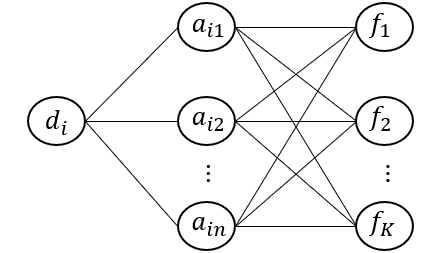
\includegraphics[width=90mm, height=50mm]{Graphics/basic_graph.png}
        \caption{Estructura de grafo propuesta}
        \label{fig: basic-graph}
    \end{figure}
\end{center}
}


\section{Tareas de aprendizaje de m\'aquinas}

El enfoque general para la resoluci\'on del problema es simular el proceso de
construcci\'on de un gr\'afico en un lenguaje de visualizaci\'on.

\begin{itemize}
    \item Seleccionar un atributo del conjunto de datos
    \item Seleccionar secuencialmente las opciones deseadas en la configuraci\'on gr\'afica de la visualizaci\'on: \begin{itemize}
        \item \bf Eje : x, y
        \item \bf Marca : barra, l\'inea, punto
        \item \bf Color : rojo, verde, azul
    \end{itemize}
\end{itemize}

Para generar el gr\'afico el usuario resuelve una serie de problemas de decisi\'on sobre las configuraciones gr\'aficas,
por este motivo dado un lenguaje de visualizaci\'on $\mathcal{C}$ con configuraciones gr\'aficas $C_1, C_2, ..., C_n$
definimos una tarea de aprendizaje de m\'aquinas por cada configuraci\'on $C_i$.

Es importante resaltar que se consideraron dos tipos de configuraciones gr\'aficas: las asociadas
a los atributos (p.e. eje, color, marca) y las asociadas al conjunto de datos (p.e. utilizaci\'on de leyendas y cuadr\'iculas).
La primeras dos tareas propuestas est\'an enfocadas a configuraciones de atributos y la tarea restante se utiliza para
las configuraciones de los conjuntos de datos.

\subsection{Problema de clasificaci\'on de v\'ertices}

Sean un grafo $G = (V,E)$ con $V = V_D \cup V_A \cup V_F$ y $E = E_{DA} \cup E_{AF}$, una configuraci\'on
gr\'afica $C$ y un conjunto $\mathcal{L}$ de etiquetas tal que existe una funci\'on biyectiva $f : \mathcal{L} \to C$.
Dado un conjunto de v\'ertices ${V_D}_l \subset V_D $ los cuales est\'an etiquetados el objetivo es aproximar la funci\'on
$h : V_D \to \mathcal{L}$ para inferir las
etiquetas para el conjunto $V_D \setminus {V_D}_l$ de v\'ertices no etiquetados. 

\subsection{Problema de predicci\'on de aristas}

Para este problema se modific\'o la arquitectura del grafo mostrada en la imagen \ref{fig: basic-graph}
a\~nadiendo el conjunto de v\'ertices $V_C$ el cual representa las posibles opciones de una configuraci\'on $C_i$ y
el conjunto de aristas $E_{AC}$ las cuales representan la utilizaci\'on una opci\'on para codificar un atributo.

\begin{figure}[h!]
    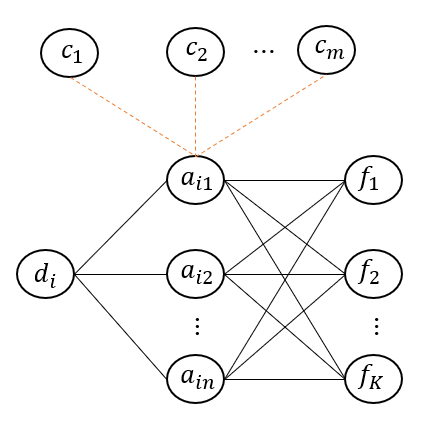
\includegraphics[width=85mm, height=65mm]{Graphics/link_pred_graph.png}
    \caption{Estructura de grafo propuesta para el problema de predicci\'on de aristas}
    \label{fig: link-pred-graph}
\end{figure}

Sean un grafo $G = (V,E)$ con $V = V_D \cup V_A \cup V_F \cup V_C$ y $E = E_{DA} \cup E_{AF} \cup E_{AC}$,
una configuraci\'on gr\'afica $C$ y $E_{AC}^*$ el conjunto de todas las posibles aristas entre los conjuntos de v\'ertices $V_A$ y $V_C$.
El objetivo es aproximar una funci\'on de probabilidad $p : E_{AC}^* \to [0,1]$ la cual indique la probabilidad de que una arista
entre un elemento $V_A$ y un elemento de $V_C$ pertenezca al grafo.

\subsection{Problema de clasificaci\'on de grafos}

Sean $C$ una configuraci\'on gr\'afica, $\mathcal{L}$ un conjunto de etiquetas y
una funci\'on biyectiva $f : \mathcal{L} \to C$. Dado un conjunto
de grafos etiquetados $\{(G_1, l_1), (G_2, l_2),..., (G_n, l_n)\}$, $l_i \in \mathcal{L} : 1 \leq i \leq n$ 
el objetivo es aproximar una funci\'on $h : \mathbb{G} \to \mathcal{L}$ donde
$\mathbb{G}$ es el espacio de todos los posibles grafos.



\chapter{Propuesta}\label{chapter:proposal}

El enfoque utilizado en este trabajo 

\section{M\'odulos del sistema}

El proceso comienza con la obtenci\'on de un conjunto de datos
ya existente del cual se quieren recomendar las configuraciones
gr\'aficas para visualizarlo. 

Los atributos de este conjunto de datos son transformados en vectores de caracter\'isticas
los cuales describen estos atributos mediante el c\'omputo de
m\'etricas estad\'isticas.

Luego los valores de las componentes de estos vectores son
discretizados y transformados en un grafo de conocimiento. Este
grafo es bipartito donde un conjunto de v\'ertices representa
los atributos del conjunto de datos y el otro conjunto representa
los posibles valores de las m\'etricas estad\'isticas utilizadas para
describirlos.

Luego este grafo es utilizado como la entrada de una red neuronal
artificial encargada de predecir la clase a la cual pertenencen los
v\'ertices del conjunto asociado a los atributos.

Definiendo una funci\'on de mapeo entre el espacio de clases existentes en este problema 
de clasificaci\'on y los posibles valores de las configuraciones gr\'aficas
disponibles se obtiene un sistema capaz de seleccionar de forma autom\'atica
configuraciones gr\'aficas para conjuntos de datos.


\begin{figure}[h!]
    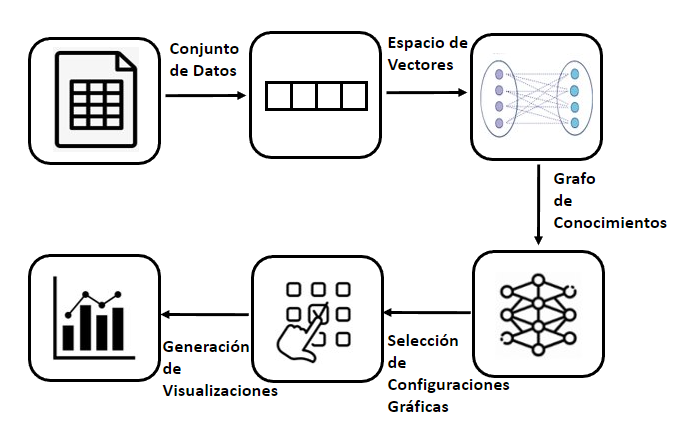
\includegraphics[width=\linewidth]{Graphics/simple_pipeline.png}
    \caption{Flujo de datos de la soluci\'on propuesta}
    \label{fig: flow_chart_sol}
\end{figure}


\subsection{M\'odulo de extraci\'on de caracter\'isticas}

El primer paso se encarga de transformar la entrada del sistema a un
espacio com\'un de $K$ dimensiones. Este proceso se realiza con el
objetivo reducir la heterogeneidad de los datos de entrada que utiliza
el modelo, debido a que los posibles conjuntos de datos a analizar
pueden provenir de distintos dominios del conocimiento humano (Medicina, Econom\'ia, etc...) \cite{vartak2017towards}.

La reducci\'on de dimensi\'on de un conjunto de datos se realiza mediante
la caracterizaci\'on de sus atributos. En este trabajo se decidi\'o caracterizar
los atributos mediante el uso de m\'etricas estad\'isticas el cual ha sido
un enfoque ampliamente usado en la literatura \cite{key2012vizdeck} \cite{vartak2014seedb} \cite{demiralp2017foresight} \cite{qian2020ml}.

Tambi\'en se toman en especial consideraci\'on problemas comunes
enmarcados dentro del an\'alisis de datos como la existencia de datos faltantes \cite{schafer2002missing}
y el soporte para distintos tipos de datos. Para ello se realiza un preprocesamiento
antes de calcular los estad\'isticos en el cual se realiza la inferencia de los tipos de datos utilizados
y la imputaci\'on de datos faltantes.

\subsection{M\'odulo de construcci\'on de grafos}

Despu\'es de obtener un conjunto de vectores de caracter\'isticas se realiza un proceso
de discretizaci\'on de las componentes de los vectores, esto tiene como objetivo aumentar
la densidad del espacio sobre el que se definen los atributos de los conjuntos de datos haciendo que 
el grafo resultante sea m\'as denso.
Cada componente es discretizada mediante la creaci\'on de intervalos que particionan el
rango de valores que puede tomar dicha componente. Para discretizar los
valores se utiliz\'o el algoritmo MDLP \cite{fayyad1993multi} el cual puede
inferir la cantidad de intervalos en que deben ser particionados los valores
bas\'andose en la distribuci\'on de los datos. Este algoritmo fue utilizado con
\'exito para esta tarea en \cite{li2021kg4vis}.

Luego se procede a construir el grafo de conocimiento, para ello se definen los conjuntos
de entidades $V_A$ que representa los atributos y $V_F$ el cual representa los posibles
rangos de valores para las distintas caracter\'isticas de los vectores. La relaci\'on entre
estos conjuntos se establece con el conjunto de aristas $E_{AF}$. Finalmente se
obtiene el grafo bipartito $G = (V_A \cup V_F, E_{AF})$.

En la literatura existen representaciones alternativas luego de la discretizaci\'on. \cite{qian2020ml} 
utiliza \textit{One Hot encoding} para representar la pertenencia
a intervalos de cada una de las m\'etricas de los atributos. Sin embargo, esto provoc\'o un 
aumento de la dimensi\'on de los vectores de caracter\'isticas lo cual conllev\'o
a emplear redes neuronales de mayores recursos.

\subsection{M\'odulo de modelos GRL}

\subsection{M\'odulo de generaci\'on de visualizaciones}